%
% fig-polar.tex -- Polarkoordinaten sind orthogonal
%
% (c) 2025 Prof Dr Andreas Müller
%
\begin{figure}
\centering
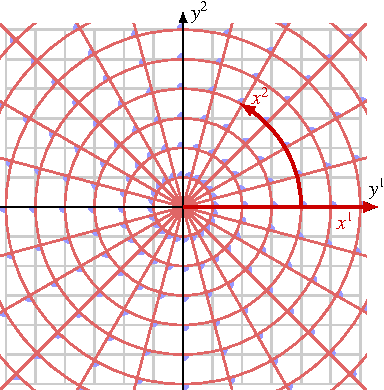
\includegraphics{papers/diffortho/images/polar.pdf}
\caption{Polarkoordinaten $(x^1,x^2)$ haben orthogonale Koordinatenlinien
({\color{darkred}rot})
und sind daher {\em orthogonale} Koordinaten.
\label{diffortho:fig:polar}}
\end{figure}
